\section{Description Logic}
\begin{itemize}
	\item Description Logic is the logic for ontologies
	\item Is more expressive than propositional logic, but less than first-order logic (DL is subsumed by FOL as classes are unary predicates and relations binary)
	\item We limit our discussion to the $\mathcal{ALC}$ description logic (\textit{Attributive Concept Language with Complements})
\end{itemize}
\subsection{Ontologies}
\begin{itemize}
	\item Organizing knowledge in a way that is useful for people
	\item Fundamental elements of ontologies
	\begin{itemize}
		\item \textit{Class}/\textit{Type}/\textit{Concept}: name + set of properties that describe certain set of individuals
		\item \textit{Instances}: members of the set defined by the class
		\item \textit{Property}/\textit{Relation}: assert facts about the instances/relation between classes
	\end{itemize}
	\item The backbone of every ontology is a type-/class-hierarchy where multi-parent inheritance is possible
	\item Axioms that need to be formalized in a logic for ontologies:
	\begin{itemize}
		\item Two classes are equivalent iff they have the same individuals and same definition
		\item The intersection and union of classes
		\item A class can be specified by either its definition or enumeration of all members
		\item Restriction of some or all values from the specified class
	\end{itemize}
	\item Property types/possible properties of relations:
	\begin{itemize}
		\item \textit{Symmetry}: if $a$ to $b$ by relation $r$, then $b$ to $a$ by $r$
		\item \textit{Asymmetry}: if $a$ to $b$ by relation $r$, then there can't be $b$ to $a$ by $r$
		\item \textit{Transitivity}: if $a$ to $b$ and $b$ to $c$ by relation $r$, then $a$ to $c$ by $r$
		\item \textit{Functionality}: if $a$ to $b$ and $a$ to $c$ by relation $r$, then $b$ and $c$ must be the same
		\item \textit{Inverse functionality}: if $a$ to $b$ and $c$ to $b$ by relation $r$, then $a$ and $c$ must be the same
		\item \textit{Reflexivity}: $a$ to $a$ by relation $r$ always holds
		\item \textit{Ir-reflexivity}: $a$ to $a$ by relation $r$ can never hold
		\item \textit{Inverse property}: if $a$ to $b$ by relation $r$, then $b$ to $a$ by relation $q$
	\end{itemize}
\end{itemize}
\subsection{Fundamentals of Description Logic}
\begin{itemize}
	\item A logic is defined by
	\begin{itemize}
		\item A language (``syntax'')
		\item The meaning of expressions (``semantics'')
		\item Inference (``deduction'')
	\end{itemize}
\end{itemize}
\subsubsection{Syntax}
\begin{itemize}
	\item The vocabulary of DL includes concept/class/type and role names
	\item Furthermore, we have the universal concept $\top$ (everything) and the bottom concept $\bot$ (nothing)
	\item More complex types can be set together by union $\sqcup$, intersection $\sqcap$ and complement $\lnot$
	\item Restrictions are encoded by $\exists r.C$ and $\forall r.C$. See semantics for meaning/explanation, and visualization in Figure~\ref{fig:kr_dl_restriction_operator_visualized}
	\begin{figure}[ht!]
		\centering
		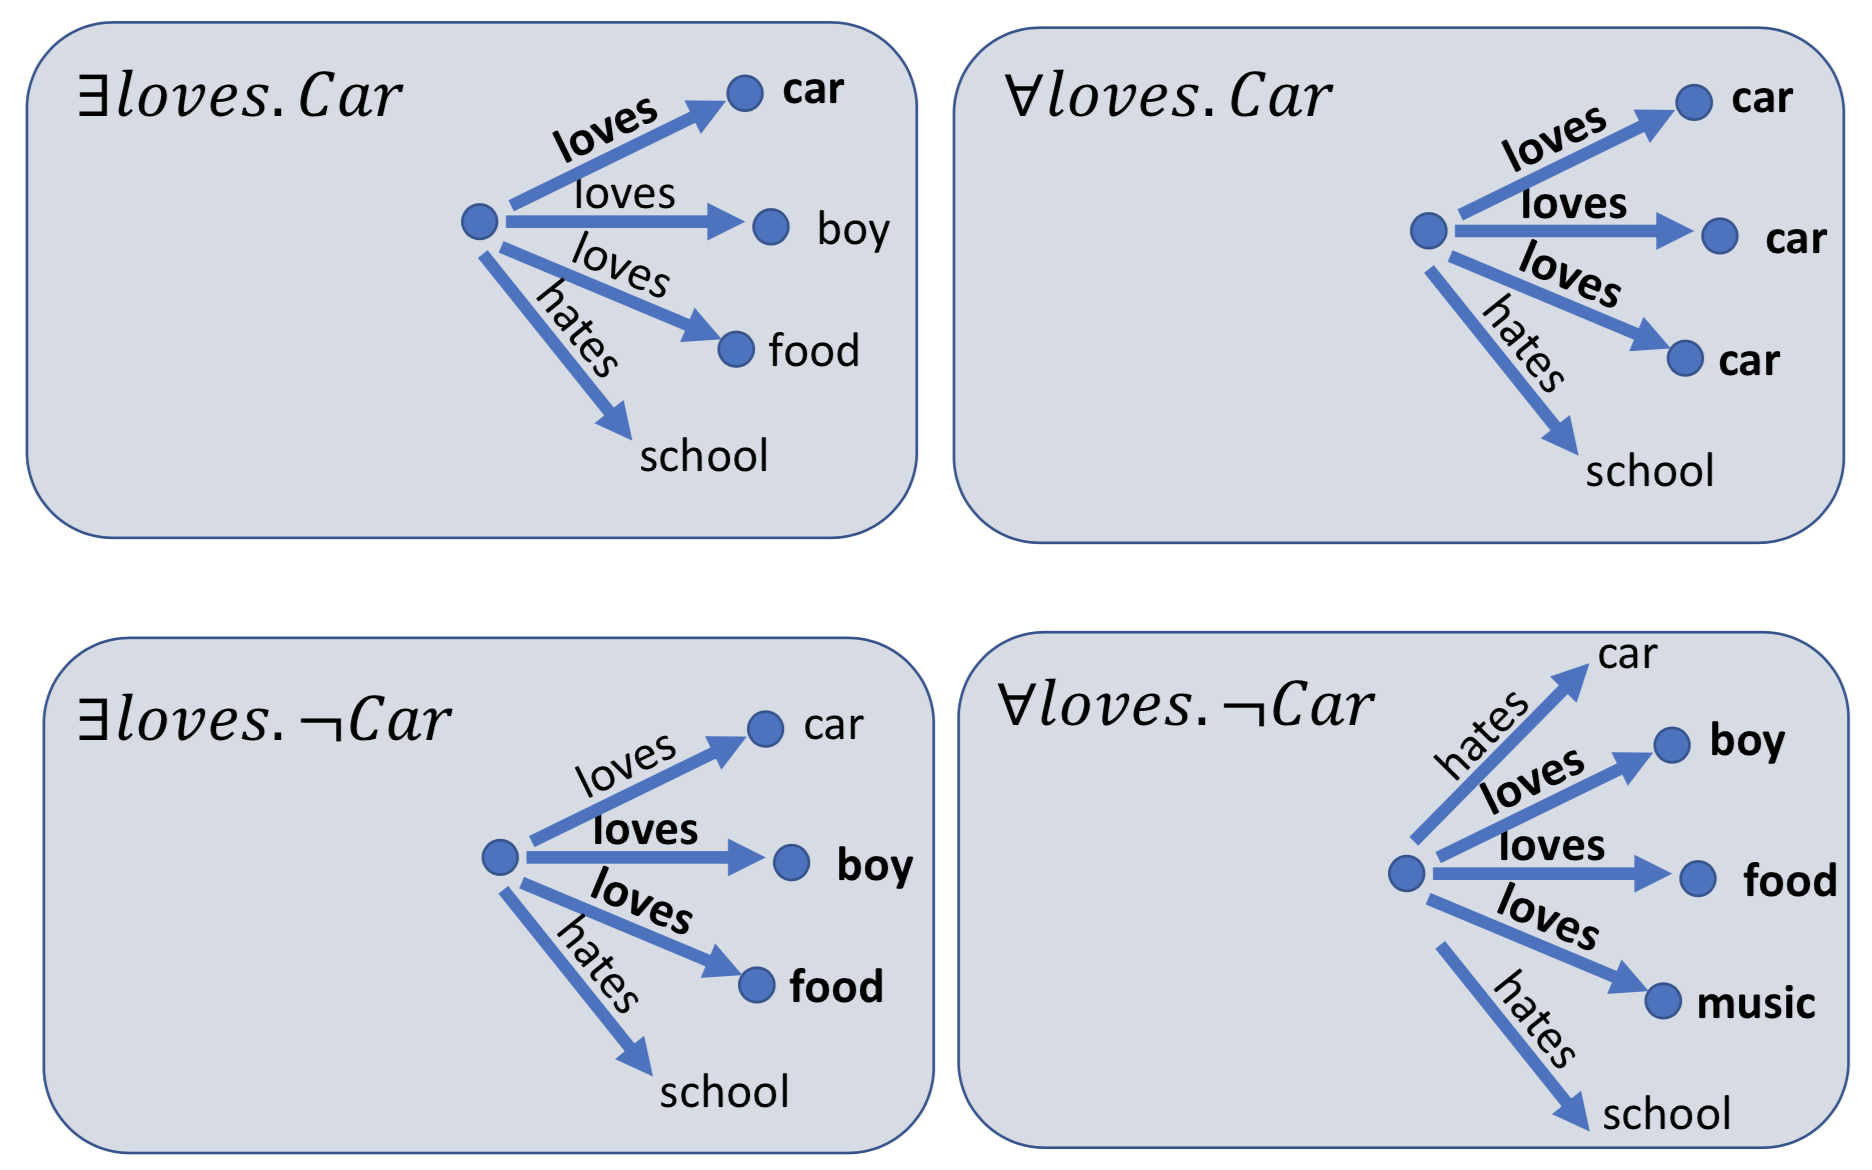
\includegraphics[width=0.4\textwidth]{figures/kr_dl_restriction_operator_visualized.png}
		\label{fig:kr_dl_restriction_operator_visualized}
		\caption{Visualization of restriction operators $\exists r.C$ and $\forall r.C$}
	\end{figure}
	\item Examples:
	\begin{itemize}
		\item $\texttt{Boys} \sqcup \texttt{Girls}$
		\item $\texttt{Girls} \sqcap \exists \texttt{owns}.\texttt{Car}$
	\end{itemize}
	\item Important for identifying concepts and roles in text. Example:
	
	``\textit{Any artwork is created by an artist. A sculpture is an artwork. A painting is an artwork that is not a sculpture. A painter is someone who painted a painting. A sculptor is someone who sculptured an artwork and only create sculptures. If an artwork is created by an artist, he has either painted or sculptured it.}''
	
	The solution would be the concepts $\left\{\texttt{Artwork}, \texttt{Artist}, \texttt{Sculptor}, \texttt{Painter}, \texttt{Painting}, \texttt{Sculpture}\right\}$, and the roles $\left\{\texttt{created}, \texttt{created\_by}, \texttt{painted}, \texttt{sculptured}\right\}$
	
	``\textit{An artwork that is not a sculpture}'': $\texttt{Artwork}\sqcap \lnot\texttt{Sculpture}$
	
	``\textit{Some who painted a painting}'': $\exists \texttt{painted}.\texttt{Painting}$
	
	``\textit{Someone who sculptured an artwork and only created sculptures}'': $\exists \texttt{sculptured}.\texttt{Artwork}\sqcap \forall \texttt{created}.\texttt{Sculpture}$
\end{itemize}
\subsubsection{Semantics}
\begin{itemize}
	\item Mathematical meaning/interpretation of syntax
	\item The interpretation function $\mathcal{I}=\left(\Delta^{\mathcal{I}}, \cdot^{\mathcal{I}} \right)$ where $\Delta^{\mathcal{I}}$ is a non-empty domain of individuals, and $\cdot^{\mathcal{I}}$ is an interpretation function that maps
	\begin{itemize}
		\item $A^{\mathcal{I}} \subseteq \Delta^{\mathcal{I}}$, i.e. concepts to subsets of $\Delta^{\mathcal{I}}$
		\item $r^{\mathcal{I}} \subseteq \Delta^{\mathcal{I}}\times \Delta^{\mathcal{I}}$, i.e. role names to subsets of $\Delta^{\mathcal{I}}\times\Delta^{\mathcal{I}}$
	\end{itemize}
	% \item Question: why has $\Delta^{\mathcal{I}}$ need to be non-empty? Is therefore a model without any individuals not allowed?
	\item $\Delta^{\mathcal{I}}$ has to be not empty as otherwise no model exists. 
	\item Thus, a concept/class/type represents a set of individuals: $\mathcal{I}(\texttt{Painter}) = \left\{\texttt{rembrandt}, \texttt{vanGogh}\right\}$
	\item Interpretation of a role/relation: $\mathcal{I}(\texttt{hasPainted}) = \left\{(\texttt{rembrandt}, \texttt{nightwatch}),(\texttt{daVinci}, \texttt{MonaLisa}) \right\}$ 
	\item $\cdot^{\mathcal{I}}$ is inductively extended over complex concept descriptions
	\begin{equation*}
		\begin{split}
			\top^{\mathcal{I}} & = \Delta^{\mathcal{I}}\\
			\bot^{\mathcal{I}} & = \emptyset\\
			(\lnot C)^{\mathcal{I}} & = \Delta^{\mathcal{I}}\setminus C^{\mathcal{I}}\\
			(C\sqcap D)^{\mathcal{I}} & = C^{\mathcal{I}} \cap D^{\mathcal{I}}\\
			(C\sqcup D)^{\mathcal{I}} & = C^{\mathcal{I}} \cup D^{\mathcal{I}}\\
			(\exists r.C)^{\mathcal{I}} & = \left\{x\in \Delta^{\mathcal{I}}\hspace{1mm}|\hspace{1mm}\exists y.(x,y)\in r^{\mathcal{I}} \wedge y\in C^{\mathcal{I}} \right\}\\
			(\forall r.C)^{\mathcal{I}} & = \left\{x\in \Delta^{\mathcal{I}}\hspace{1mm}|\hspace{1mm}\forall y.(x,y)\in r^{\mathcal{I}} \to y\in C^{\mathcal{I}} \right\}
		\end{split}
	\end{equation*}
	\begin{figure}[ht!]
		\centering
		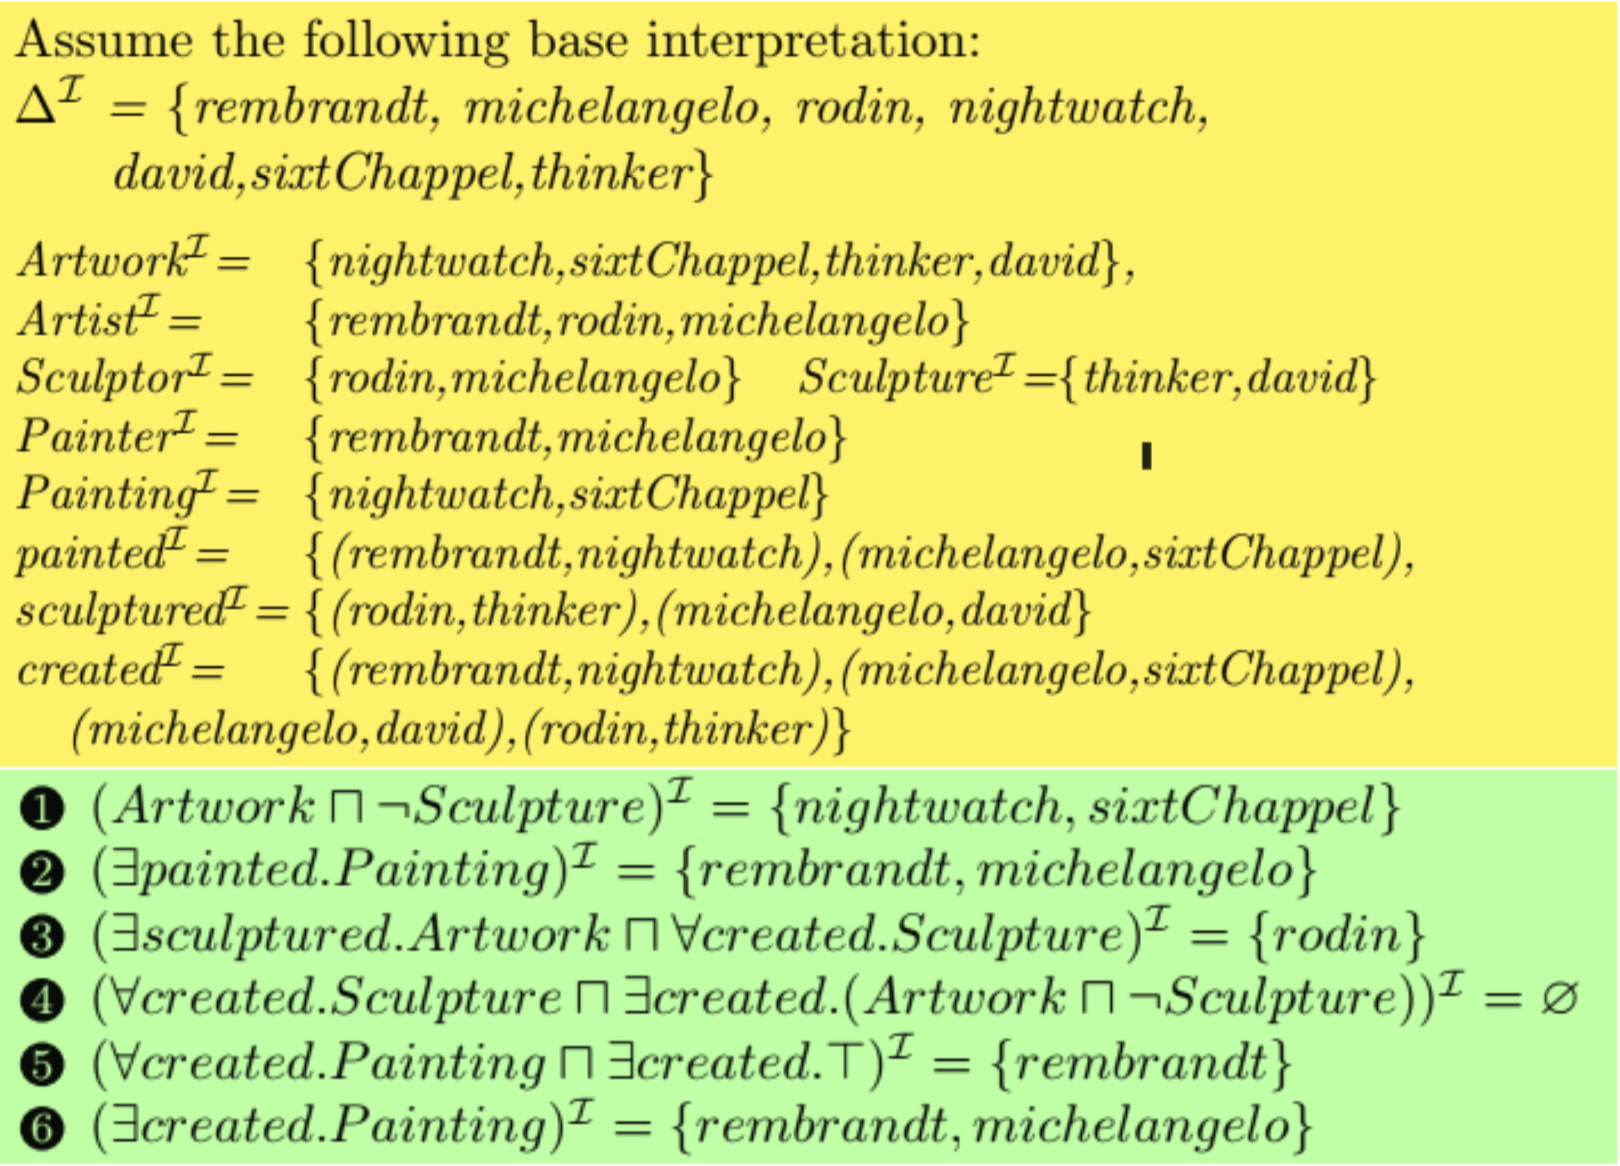
\includegraphics[width=0.4\textwidth]{figures/kr_dl_interpretation_example.png}
		\caption{Example for interpretation function $\mathcal{I}$}
	\end{figure}
	\item Note that the quantifier $\forall r.C$ also includes the empty set. To prevent this, use $\forall r.C \sqcap \exists r.\top$
	% kr_dl_interpretation_example.png
\end{itemize}
\subsection{Inference in Description Logic}
\begin{itemize}
	\item A \textbf{knowledge base} $\mathcal{K} = (\mathcal{T}, \mathcal{A}) $ consists of:
	\begin{itemize}
		\item the terminology/theory $\mathcal{T}$, that defines the general world model you can apply to any model. It summarizes the relations between concepts.
		\begin{itemize}
			\item The knowledge about relations between concepts is expressed by means of terminological axioms
			\item \textit{Concept inclusion}: $C\sqsubseteq D$ models necessary conditions for object of type $C$ 
			
			Example: $\texttt{Elephant} \sqsubseteq \texttt{Animal} \sqcap \lnot\texttt{Mouse}$
			\item \textit{Concept equivalence}: $C\equiv D$ models necessary and sufficient conditions for object $C$. Can also be written as $C \sqsubseteq D$ and $D \sqsubseteq C$
			
			Example: $\mathcal{T}$: ``\textit{painter is a human that created a painting}'' $\Rightarrow$ $\texttt{Painter} \equiv \texttt{human}\sqcap \exists\texttt{created}.\texttt{Painting}$
		\end{itemize}
		\item the assertions $\mathcal{A}$ that describes certain objects and the sets that are defined by $\mathcal{T}$
		\begin{itemize}
			\item Knowledge about individuals in the domain expressed in terms of the vocabulary is specified by means of assertional axioms 
			\item \textit{Concept assertion}: $a : C$ models that individual $a$ is of class $C$ 
			
			Example: $\texttt{dumbo}: \texttt{Elephant}$
			\item \textit{Role assertions}: $(a, b) : r$ models that individual $a$ is related to individual $b$ by the role $r$
			
			Example: $(\texttt{daVinci}, \texttt{MonaLisa}) : \texttt{painted}$
		\end{itemize}
	\end{itemize}
	\item Definition of a \textit{\textbf{model}}
	\begin{itemize}
		\item An interpretation $\mathcal{I}$ is a \textit{model} of the $\mathcal{T}$-box iff it satisfies every terminological axiom in $\mathcal{T}$
		\item An interpretation $\mathcal{I}$ is a \textit{model} of the $\mathcal{A}$-box iff it satisfies every assertional axiom in $\mathcal{A}$
		
		Note that this just requires $\mathcal{I}$ to have the individuals and relations/assertions defined in $\mathcal{A}$
		\item Finally, an interpretation $\mathcal{I}$ is a \textit{model} of the knowledge base $\mathcal{K} = (\mathcal{T},\mathcal{A})$-box iff $\mathcal{I}$ is a model of both $\mathcal{T}$ and $\mathcal{A}$
		\item A knowledge base is called \textit{satisfiable}/\textit{consistent} iff there exists a model for it.
	\end{itemize}
	\item In general, axioms of $\mathcal{A}$- and $\mathcal{T}$-box restrict the possible models
	\item \textbf{Reasoning tasks} for $\mathcal{T}$-box
	\begin{itemize}
		\item \textit{Concept satisfiability}: Concept $C$ is satisfiable w.r.t. $\mathcal{T}$ iff there is a model $\mathcal{I}$ of $\mathcal{T}$: $C^{\mathcal{I}} \neq \emptyset$
		\item \textit{Subsumption}: check if $\mathcal{T} \models C\sqsubseteq D$. $C$ is subsumed by $D$ in $\mathcal{T}$ iff $C^{\mathcal{I}}\subseteq D^{\mathcal{I}}$ in every model $\mathcal{I}$ of $\mathcal{T}$
		\item \textit{Equivalence}: check if $\mathcal{T} \models C\equiv D$. Concepts $C$ and $D$ are equivalent in $\mathcal{T}$ iff $C^{\mathcal{I}} = D^{\mathcal{I}}$ in every model $\mathcal{I}$ of $\mathcal{T}$
		\item All $\mathcal{T}$-box problems can be reduced to concept satisfiability which is equivalent to showing that $C\sqcap \lnot D$ is unsatisfiable in $\mathcal{T}$ (see section~\ref{sec:tableau_algorithm} for Tableau algorithm to solve this)
	\end{itemize}
	\item \textbf{Reasoning tasks} for $\mathcal{A}$-box
	\begin{itemize}
		\item \textit{$\mathcal{A}$-box consistency}: $\mathcal{A}$ is consistent w.r.t. $\mathcal{T}$ iff there is a model of $\mathcal{K}$. In such a case, $\mathcal{K}$ is satisfiable.
		\item \textit{Instance checking}: check if $\mathcal{K} \models a:C$ (or respectively $\mathcal{K} \models (a,b) : r$). This holds iff for every model of $\mathcal{K}$ is a model of $a:C$
		\item \textcolor{red}{Question: don't we also need the assertion that $\mathcal{K}$ is consistent as otherwise we can prove anything for an unsatisfiable knowledge base?}
		\item \textit{Retrieval task}: given a concept $C$ and an $\mathcal{A}$-box $\mathcal{A}$, find all individuals $a$ such that $\mathcal{K}\models a:C$
		\item \textit{Realization task}: given an individual $a$ and a set of concepts, find the most specific concept $C$ such that $\mathcal{K}\models a:C$
		\item All tasks are reducible to checking $\mathcal{A}$-box consistency. We can check those by showing that $\mathcal{A} \cup \left\{a:\lnot C\right\}$ is inconsistent.
	\end{itemize}
\end{itemize}
\subsubsection{Tableau algorithm}
\label{sec:tableau_algorithm}
\begin{itemize}
	\item All reasoning tasks in $\mathcal{ALC}$ can be reduced to a single task of checking
	$\mathcal{A}$-box consistency w.r.t. $\mathcal{T}$-box.
	\item Tableau shows (un-)satisfiability by contradiction. It searches through the tree of possible models and delivers a proof iff no model exists and therefore the input inconsistent is (or otherwise returns a valid model).
	\item The general approach of Tableau is to extend the model until we find a model, or closed all branches
	\item To reduce the number of tableau proves, we assume that all concepts appear in the Negation Normal Form (NNF). Conversion rules:
	\begin{equation*}
		\begin{split}
			\lnot\left(C \cap D\right) & \Rightarrow \left(\lnot C \cup \lnot D\right)\\
			\lnot\left(C \cup D\right) & \Rightarrow \left(\lnot C \cap \lnot D\right)\\
			\lnot\exists r.C & \Rightarrow \forall r.\lnot C\\
			\lnot\forall r.C & \Rightarrow \exists r.\lnot C\\
		\end{split}
	\end{equation*}
	\item A \textit{\textbf{branch}} of a tableau is a set of $\mathcal{A}$-box assertions. For any branch $S$, the following rules apply:
%	\begin{figure}[ht!]
%		\hspace{10mm}
%		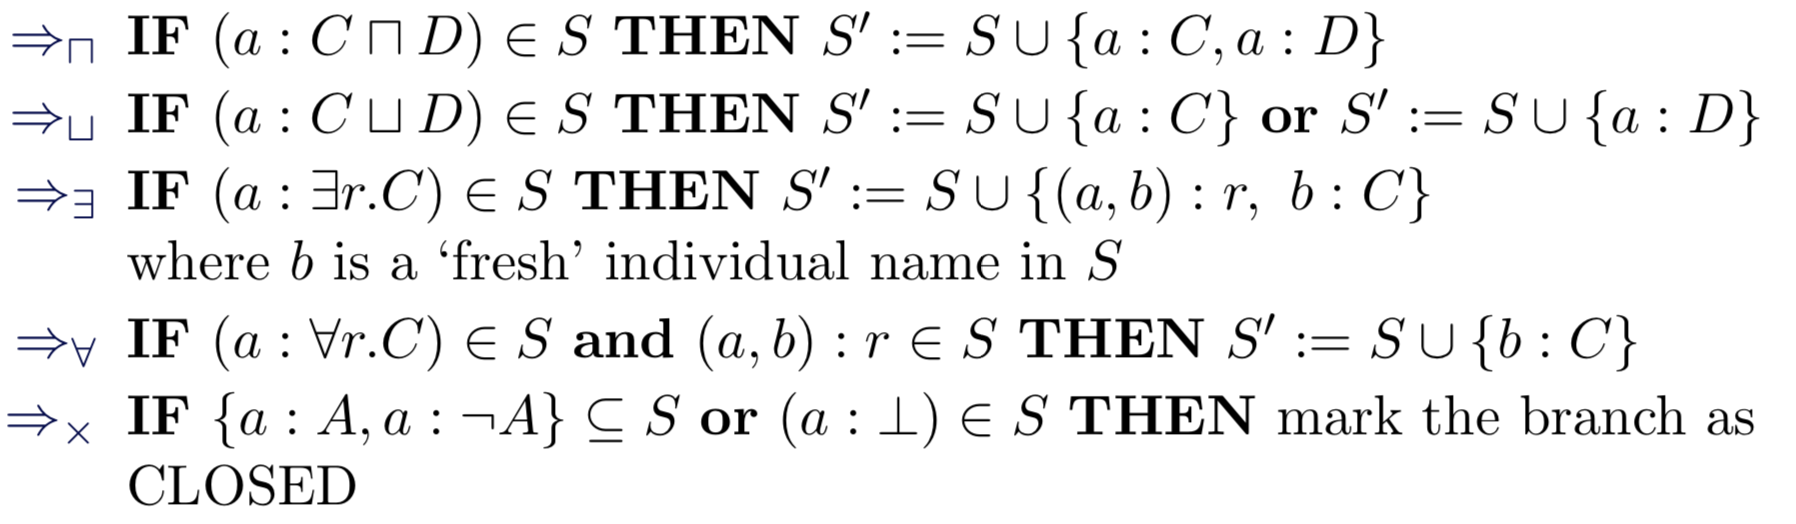
\includegraphics[width=0.6\textwidth]{figures/kr_dl_tableau_rules.png}
%	\end{figure}
	\begin{itemize}
		\item \textbf{IF} $(a:C\sqcap D)\in S$ \textbf{THEN} $S' := S \cup \left\{a:C, a:D\right\}$
		\item \textbf{IF} $(a:C\sqcup D)\in S$ \textbf{THEN} $S' := S \cup \left\{a:C\right\}$ \textbf{or} $S' := S \cup \left\{a:D\right\}$
		\item \textbf{IF} $(a:\exists r.C)\in S$ \textbf{THEN} $S' := S \cup \left\{(a,b):r, b:C\right\}$ where $b$ is a ``fresh'' individual name in $S$
		\item \textbf{IF} $(a:\forall r.C)\in S$ \textbf{and} $(a,b):r \in S$ \textbf{THEN} $S' := S \cup \left\{b:C\right\}$
		\item \textbf{IF} $\left\{a:C, a:\lnot C\right\}\subseteq S$ \textbf{THEN} mark branch as CLOSED (unsatisfiable)
	\end{itemize}
	\item To check for satisfiability, we assume that there is an individual of that given concept. Try to show that this leads to an contradiction.
	\item Example: \textit{show that $\exists r.A \sqcap \exists r.B$ is subsumed by $\exists r.(A\sqcap B)$}
	\begin{enumerate}
		\item Write expression as concept: $\exists r.A \sqcap \exists r.B \sqsubseteq \exists r.(A\sqcap B)$
		\item Negate concept (proof by contradiction): $\exists r.A \sqcap \exists r.B \sqcap \lnot \exists r.(A\sqcap B)$
		\item Rewrite concept in NNF: $\exists r.A \sqcap \exists r.B \sqcap \forall r.(\lnot A\sqcup \lnot B)$
		\item Assume $\mathcal{A}$-box $\mathcal{A}=\left\{a: \exists r.A \sqcap \exists r.B \sqcap \forall r.(\lnot A\sqcup \lnot B)\right\}$ and search for a model
%		\begin{itemize}
%			\item $a: \exists r.A$, $a: \exists r.B$, $a: \forall r.(\lnot A\sqcup \lnot B)$
%			\item $(a,b):r$, $b:A$, $(a,c):r$, $c:B$
%			\item $b:(\lnot A\sqcup \lnot B)$, $c:(\lnot A\sqcup \lnot B)$
%			
%		\end{itemize}
% kr_dl_tableau_proof_example.png
		\begin{figure}[ht!]
			\hspace{30mm}
			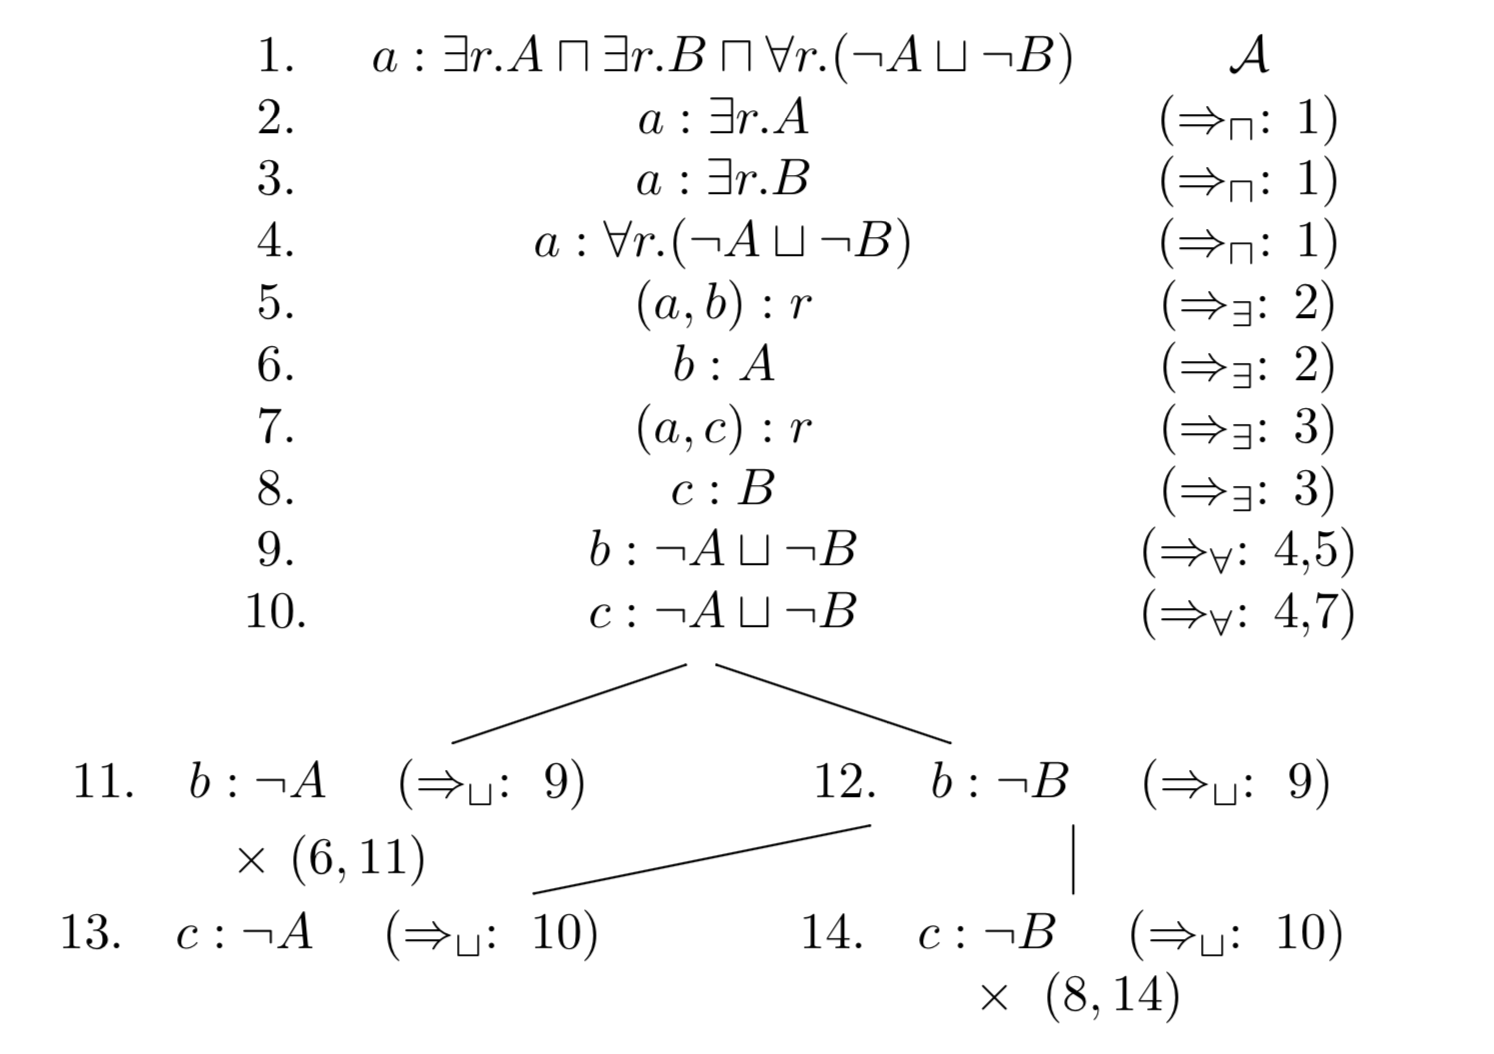
\includegraphics[width=0.5\textwidth]{figures/kr_dl_tableau_proof_example.png}
		\end{figure}
		\item Step 13 shows the valid model where $\Delta^{\mathcal{I}}=\left\{a,b,c\right\}$, $A^{\mathcal{I}}=\left\{b\right\}$, $B^{\mathcal{I}}=\left\{c\right\}$, $r^{\mathcal{I}}=\left\{(a,b), (a,c)\right\}$ $\Rightarrow$ the negated concept is satisfiable and thus proves the hypothesis to be wrong
		
		If we would not have been able to construct a model, the hypothesis would be correct 
	\end{enumerate}
	\item Note that the tableau algorithm is sound (if algorithm finds a proof, then statement is correct) and complete (if statement is correct, the algorithm finds a proof).
\end{itemize}
\subsubsection{Reasoning with non-empty $\mathcal{T}$-box}
\begin{itemize}
	\item The tableau algorithm can be extended in order to support terminology axioms of the $\mathcal{T}$-box
	\item Input preprocessing
	\begin{itemize}
		\item Replace every $C\equiv D \in \mathcal{T}$ with $C\sqsubseteq D$ and $D\sqsubseteq C$
		\item Replace every $C\sqsubseteq D \in \mathcal{T}$ with $\top \equiv NNF(\lnot C \sqcup D)$
		\item Add all concepts/formula of $\mathcal{T}$ to the root $S_0$ of the tableau
	\end{itemize}
	\item Extend the tableau rules by the following:
	\begin{itemize}
		\item \textbf{IF} $(\top \equiv C) \in S$ \textbf{and} an individual $a$ occurs in $S$ \textbf{THEN} $S' := S\cup\left\{a:C\right\}$
	\end{itemize}
	\item Example:
	\begin{figure}[ht!]
		\hspace{10mm}
		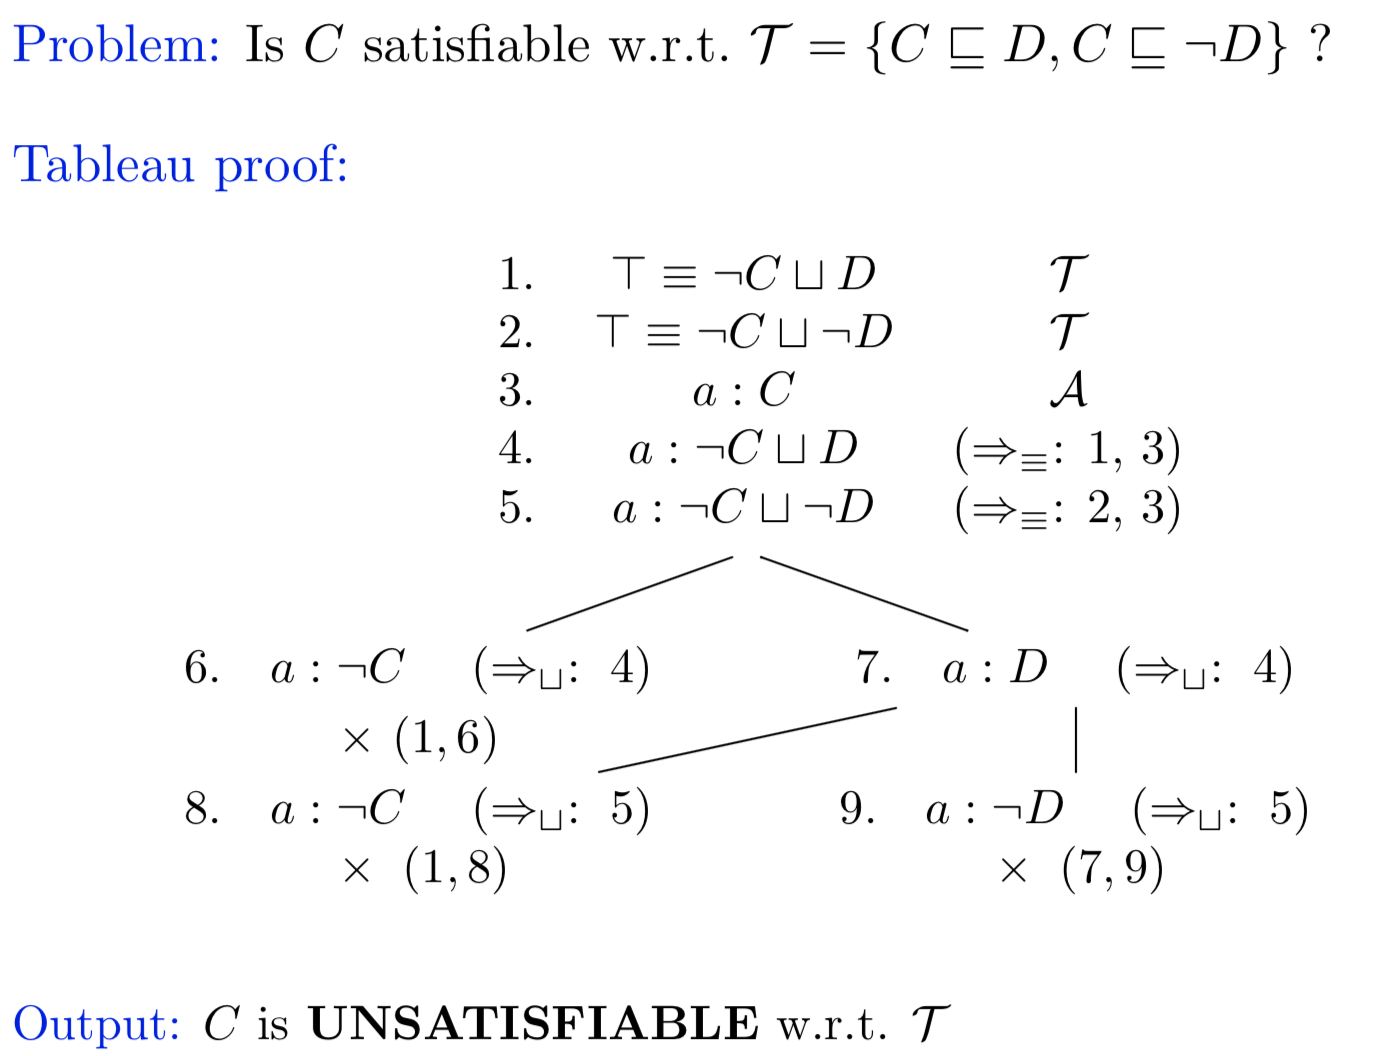
\includegraphics[width=0.5\textwidth]{figures/kr_dl_tableau_nonempty_tbox_example.png}
	\end{figure}
	\item In case of reasoning with non-empty $\mathcal{T}$-box, the tableau algorithm is not guaranteed to terminate (rules in the form of $\top\equiv ...\exists r.C...$ can lead to an infinite loop)
	\item Solution: Detect cycles and prevent further application of the $\Rightarrow_{\exists}$ rule. This is achieved by a special blocking rule:
	\begin{itemize}
		\item \textbf{IF} $b$ is a (possibly indirect) successor of $a$ in $S$ \textbf{and} it is the case that: $$\left\{C\hspace{1mm}|\hspace{1mm} b:C \in S\right\} \subset \left\{D\hspace{1mm}|\hspace{1mm} a:D \in S\right\} $$
		
		\textbf{THEN} mark $b$ as BLOCKED by $a$ in $S$ and do not apply $\Rightarrow_{\exists}$ rule to $b$.
	\end{itemize}
	\item Example:
	\begin{figure}[ht!]
		\hspace{10mm}
		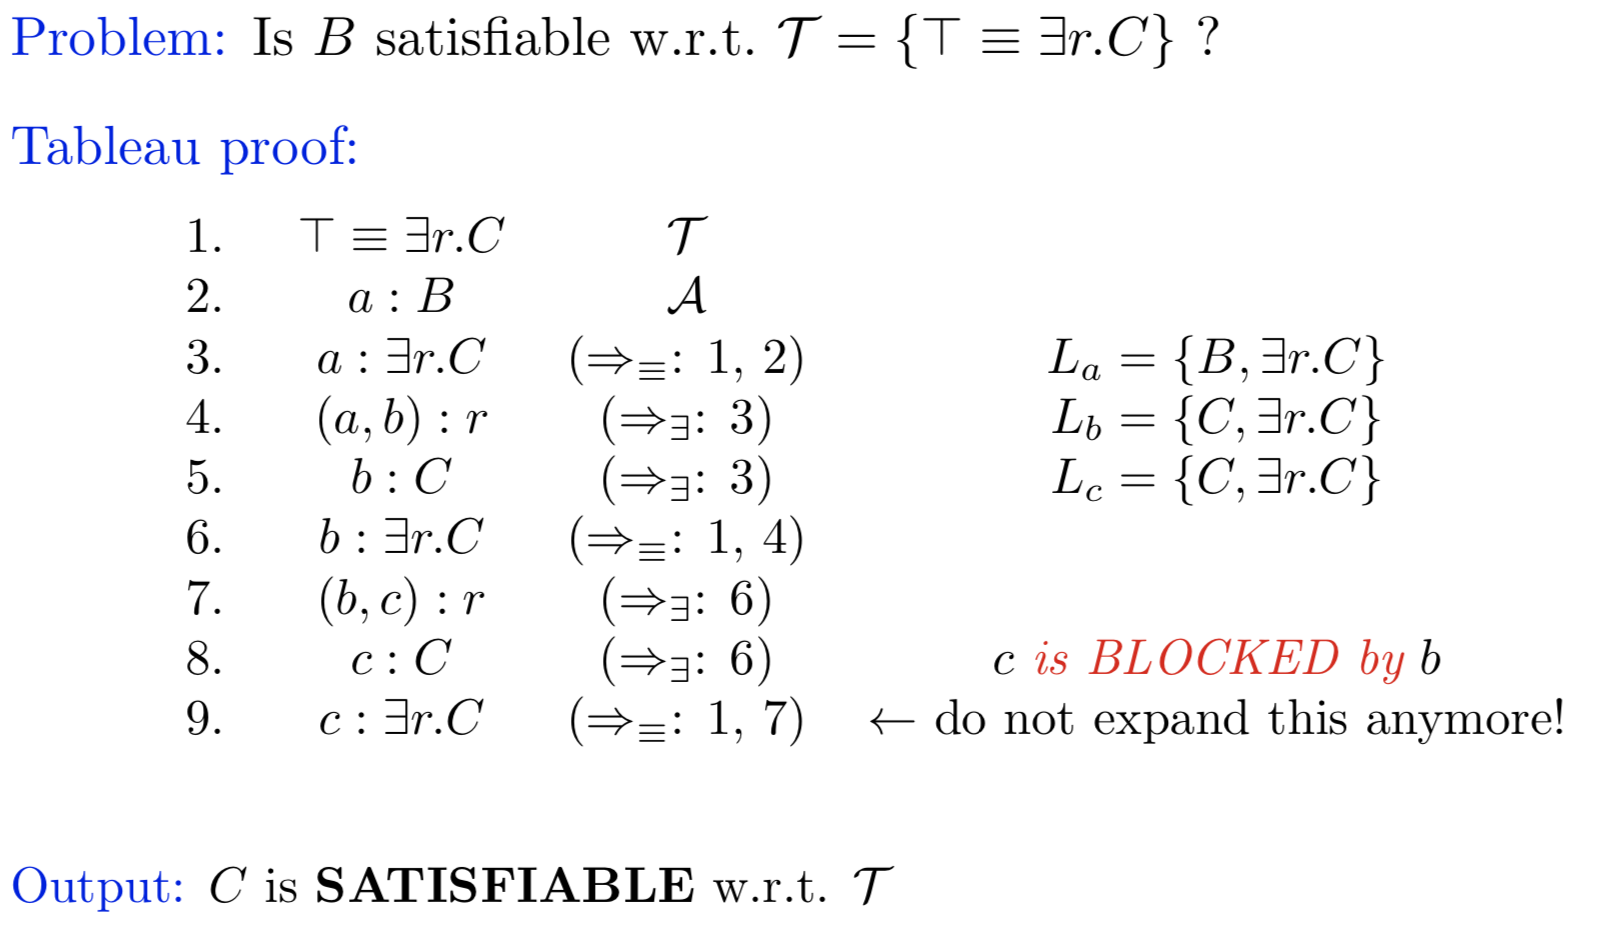
\includegraphics[width=0.5\textwidth]{figures/kr_dl_tableau_blocking_example.png}
	\end{figure}
	\item Note that we can only apply the blocking rule if no other rules apply anymore on that branch.
\end{itemize}